\documentclass[11pt]{article}
\usepackage[margin=1in]{geometry}
\usepackage{amsmath,amssymb,amsthm,graphicx,booktabs,array,hyperref}
\newtheorem{lemma}{Lemma}
\renewcommand{\topfraction}{0.9}
\renewcommand{\bottomfraction}{0.8}
\renewcommand{\textfraction}{0.1}
\renewcommand{\floatpagefraction}{0.85}
\setcounter{totalnumber}{4}
\title{A Low-Thrust Orbital Network over the Costate Catalogs:\\ what Braik and Ross's framing says about certified min-time transfers}
\author{Michael Casey}
\date{November 2026}
\begin{document}
\maketitle

\section{Motivation}
Braik and Ross~\cite{braik2026} build a weighted graph of 13 planar Earth--Moon periodic orbits on
one Jacobi level. An edge between two orbits is scored by the overlap of their reachable sets under
heading-change impulses, with turn cost $2v\sin(|\delta|/2)$ and the budget split symmetrically,
half at each end. From that graph they read hubs (the orbit C32 among them), relay orbits, and three
budget-dependent stages of connectivity. Their stability reading is that unstable orbits share a
chaotic sea and connect cheaply, while stable ones sit inside tori and are hard to reach or leave.
We care because the same question can be put to our DRO $\to$ tulip transfers, whose direct
min-time catalog continuation closes down to 0.09~N and stalls at a basin wall between 0.09 and
0.067~N (the 70~mN phase library is certified on separately seeded branches): does the network view, and does orbit stability,
say anything about the certified min-time transfers we already hold? This note lifts both ideas onto
the four costate catalogs with no proxies and no new solves.

\section{Their problem and ours}
Table~\ref{tab:problems} sets the two problems side by side. The difference that matters most for
relays is not in the table: their direct cost is the cost of one restricted maneuver class, while
ours is the optimum of an optimal control problem whose feasible set already contains every relay
route. The lemma makes that precise.

\begin{table}[tbp]
\centering\small
\begin{tabular}{@{}lll@{}}
\toprule
 & Braik and Ross~\cite{braik2026} & this note \\
\midrule
dynamics & planar CR3BP & spatial CR3BP \\
energy & one Jacobi level & Jacobi gaps $\Delta C_J$ from $-0.16$ to $0.33$ \\
control & energy-preserving heading impulses & mass-varying continuous thrust \\
edge cost & reachable-set overlap (proxy) & accepted min-time extremals \\
certification & none (proxy cost) & multiple shooting, conjugate test, hypothesis gates \\
phase & future work & $6\times 6$ departure/arrival phasing grid per sheet \\
\bottomrule
\end{tabular}
\caption{The two problems.}
\label{tab:problems}
\end{table}

\begin{lemma}[unrestricted versus relay-constrained optimum]
Let $\mathcal{F}_{AB}$ be the set of feasible trajectories of a specified $A \to B$ optimal control
problem, including the spacecraft mass and every boundary and path constraint. Let
$\mathcal{R}_{ACB} \subseteq \mathcal{F}_{AB}$ be the subset of trajectories that pass through the
relay orbit $C$ with compatible full states at every join and no relay-only operation. Then for the
same cost functional $J$,
\[
\inf_{x \in \mathcal{F}_{AB}} J[x] \;\le\; \inf_{x \in \mathcal{R}_{ACB}} J[x].
\]
\end{lemma}
\begin{proof}
$\mathcal{R}_{ACB}$ is a subset of $\mathcal{F}_{AB}$, and an infimum over a set is no larger than
the infimum over any of its subsets.
\end{proof}

The lemma is a statement about global infima, not about the costs returned by particular direct or
relay solution procedures. A multileg advantage in Braik and Ross is relative to their restricted
direct-maneuver class; it is not a comparison against the global optimum over a feasible set that
already contains those multileg trajectories. A relay witness below the termination thrust of our
computed direct branch would establish another feasible unrestricted transfer; it would diagnose a
limitation of that branch or of the search, not passage through a proven global feasibility barrier.

The full-state hypothesis includes the mass, and the catalogs solve every leg from the same initial
mass. A leg solved from $m_0$ can be flown from the previous leg's arrival mass $m_1$ by scaling its
thrust and mass histories by $q = m_1/m_0 \le 1$: the acceleration $F/m$ and the path are unchanged,
the mass equation still holds, and the thrust bound is respected. The assembled route is feasible
without a new solve; the scaled leg is not thereby optimal or certified for the changed
initial-mass problem.

\section{The data}\label{sec:data}
Four min-time catalogs supply 56 sheets (Table~\ref{tab:catalogs}). A sheet is one (departure orbit,
arrival orbit) pair; each holds a $6 \times 6$ grid of departure and arrival phases, at fractions
$0, 1/6, \dots, 5/6$ of each orbit's period from the same initial-state origin in every catalog, on
each rung of the thrust ladder $[15\ 12\ 10\ 7\ 5\ 3\ 2\ 1.5\ 1\ 0.75\ 0.5]$~N. A cell is
\emph{accepted} when it is solved, passes the conjugate-point test (\texttt{conj\_pass} $=1$; the
stored $-1$ means ``not run'' and is not a pass) and has positive margins on the three hypothesis
gates ($\min|\lambda_v|$, $Q_{mt}$, $\dim S = 1$). Every count, minimum, plane and route below is
over accepted cells.

\begin{table}[tbp]
\centering\small
\begin{tabular}{@{}llrl@{}}
\toprule
catalog & departure orbits & sheets & arrival orbits \\
\midrule
\texttt{DRO\_tulip}  & DRO $\tau = 0.5, 1, 2, 3$ & 16 & tulip $N_p = 5, 7, 9, 12$ \\
\texttt{HALO\_tulip} & L2 south halo $\tau = 1.75, 2.2, 2.8, 3.4$ & 16 & the same tulips \\
\texttt{DPO\_tulip}  & DPO $\tau = 1, 2, 3, 4$ & 16 & the same tulips \\
\texttt{HALO\_HALO}  & L1 south halo $\tau = 1.8037, 2.7433$ & 8 & the four L2 halos \\
\bottomrule
\end{tabular}
\caption{The four catalogs: 56 sheets over 18 distinct orbits.}
\label{tab:catalogs}
\end{table}

Summed over the 56 sheets, the solved and accepted cells per rung are
\begin{center}\small
\begin{tabular}{@{}lrrrrrrrrrrr@{}}
\toprule
rung [N] & 15 & 12 & 10 & 7 & 5 & 3 & 2 & 1.5 & 1 & 0.75 & 0.5 \\
\midrule
solved   & 1579 & 1688 & 1674 & 1640 & 1623 & 1572 & 1516 & 1384 & 1124 & 1090 & 940 \\
accepted & 1578 & 1688 & 1674 & 1640 & 1622 & 1570 & 1512 & 1381 & 1118 & 1069 & 898 \\
\bottomrule
\end{tabular}
\end{center}
Some cells are refuted or gated
at most rungs (none at 12, 10 and 7~N), most at 0.75 and 0.5~N. Every cell solved at 0.5~N is solved at 1~N, so the
solved sets are nested between the two rungs the study uses; four cells are accepted at 0.5~N but
not at 1~N, so the accepted sets are not. Along the whole ladder the solved sets are not nested:
593 cells are solved at a rung and open one rung shallower, and the 15~N starting rung holds fewer
solved cells than 12~N. That is solver coverage at the top of the ladder. An unaccepted cell or rung
is unresolved, never a demonstrated infeasibility.

Table~\ref{tab:nodes} lists the 18 orbits. The stability index is
$\sigma = \ln|\lambda|_{\max}/T$ from the monodromy matrix, set to exactly zero when
$|\lambda|_{\max} < 1 + 10^{-3}$; a zero means no resolved exponential instability in the computed
multipliers. All four DROs, all four tulips, DPO $\tau=1$ and L2 halo $\tau=2.2$ are stable in that
sense. The symplectic pairing $|\lambda|_{\max}|\lambda|_{\min} = 1$ holds to $2.0\times10^{-9}$ and
$\det M = 1$ to $3.0\times10^{-9}$ on all 18 orbits, and the node periods match the catalogs to
$8.9\times10^{-16}$.

\begin{table}[tbp]
\centering\footnotesize
\begin{tabular}{@{}lrrrrcrrrr@{}}
\toprule
orbit & $T$ [ND] & $C_J$ & $|\lambda|_{\max}$ & $\sigma$ & stable & in & out & in-str & out-str \\
\midrule
\texttt{dro\_tau0.5}       & 0.5000 & 3.17747 & 1.0000 & 0      & 1 & 0  & 4 & 0     & 2.206 \\
\texttt{dro\_tau1}         & 1.0000 & 3.05758 & 1.0000 & 0      & 1 & 0  & 4 & 0     & 2.322 \\
\texttt{dro\_tau2}         & 2.0000 & 2.97466 & 1.0000 & 0      & 1 & 0  & 4 & 0     & 2.116 \\
\texttt{dro\_tau3}         & 3.0000 & 2.93509 & 1.0000 & 0      & 1 & 0  & 4 & 0     & 1.814 \\
\texttt{halo\_L2\_tau1.75} & 1.7500 & 3.03152 & 3.0030 & 0.6284 & 0 & 2  & 4 & 1.037 & 2.855 \\
\texttt{halo\_L2\_tau2.2}  & 2.2000 & 3.01663 & 1.0001 & 0      & 1 & 2  & 4 & 0.989 & 2.949 \\
\texttt{halo\_L2\_tau2.8}  & 2.8000 & 3.02530 & 26.970 & 1.1767 & 0 & 2  & 4 & 0.908 & 2.442 \\
\texttt{halo\_L2\_tau3.4}  & 3.4000 & 3.14402 & 1051.4 & 2.0464 & 0 & 2  & 4 & 0.808 & 2.179 \\
\texttt{dpo\_tau1}         & 1.0000 & 3.20776 & 1.0000 & 0      & 1 & 0  & 4 & 0     & 2.742 \\
\texttt{dpo\_tau2}         & 2.0000 & 3.15196 & 11.479 & 1.2203 & 0 & 0  & 4 & 0     & 2.739 \\
\texttt{dpo\_tau3}         & 3.0000 & 3.11096 & 168.34 & 1.7087 & 0 & 0  & 4 & 0     & 2.544 \\
\texttt{dpo\_tau4}         & 4.0000 & 3.06634 & 796.88 & 1.6702 & 0 & 0  & 4 & 0     & 2.401 \\
\texttt{halo\_L1\_tau1.8037} & 1.8037 & 3.00186 & 4.8460 & 0.8750 & 0 & 0 & 4 & 0   & 2.046 \\
\texttt{halo\_L1\_tau2.7433} & 2.7433 & 3.17397 & 2345.7 & 2.8288 & 0 & 0 & 4 & 0   & 1.695 \\
\texttt{tulip\_Np5}        & 4.7124 & 3.14552 & 1.0000 & 0      & 1 & 12 & 0 & 6.928 & 0 \\
\texttt{tulip\_Np7}        & 5.2360 & 3.18662 & 1.0000 & 0      & 1 & 12 & 0 & 7.040 & 0 \\
\texttt{tulip\_Np9}        & 5.4978 & 3.22119 & 1.0002 & 0      & 1 & 12 & 0 & 7.534 & 0 \\
\texttt{tulip\_Np12}       & 5.7120 & 3.26775 & 1.0003 & 0      & 1 & 12 & 0 & 7.808 & 0 \\
\bottomrule
\end{tabular}
\caption{The 18 nodes. $\sigma$ in 1/ND, zero when $|\lambda|_{\max} < 1 + 10^{-3}$. The last four
columns are the in- and out-degree and the in- and out-strength at 1~N (weights $1/t_f$, $t_f$ the
minimum accepted time in days); see Section~\ref{sec:graph} for the caveat.}
\label{tab:nodes}
\end{table}

\section{The graph}\label{sec:graph}
The nodes are the 18 orbits and the 56 edges are the sheets. Each edge carries, per rung, the
accepted fraction of its 36 cells, the minimum and median $t_f$ over its accepted cells, and its
lowest accepted rung. A successful rung bounds nothing below it: the lowest accepted rung is where
the catalog's ladder stopped with a witness, not a property of the transfer. Here it is the lowest
tested rung on every edge: all 56 edges have at least one accepted cell at 0.5~N, and all 56 have
at least one at 1~N. Figure~\ref{fig:graph} draws the graph at 1~N and at
0.5~N, with width set by the accepted fraction and color by the minimum $t_f$.

\begin{figure}[tbp]
\centering
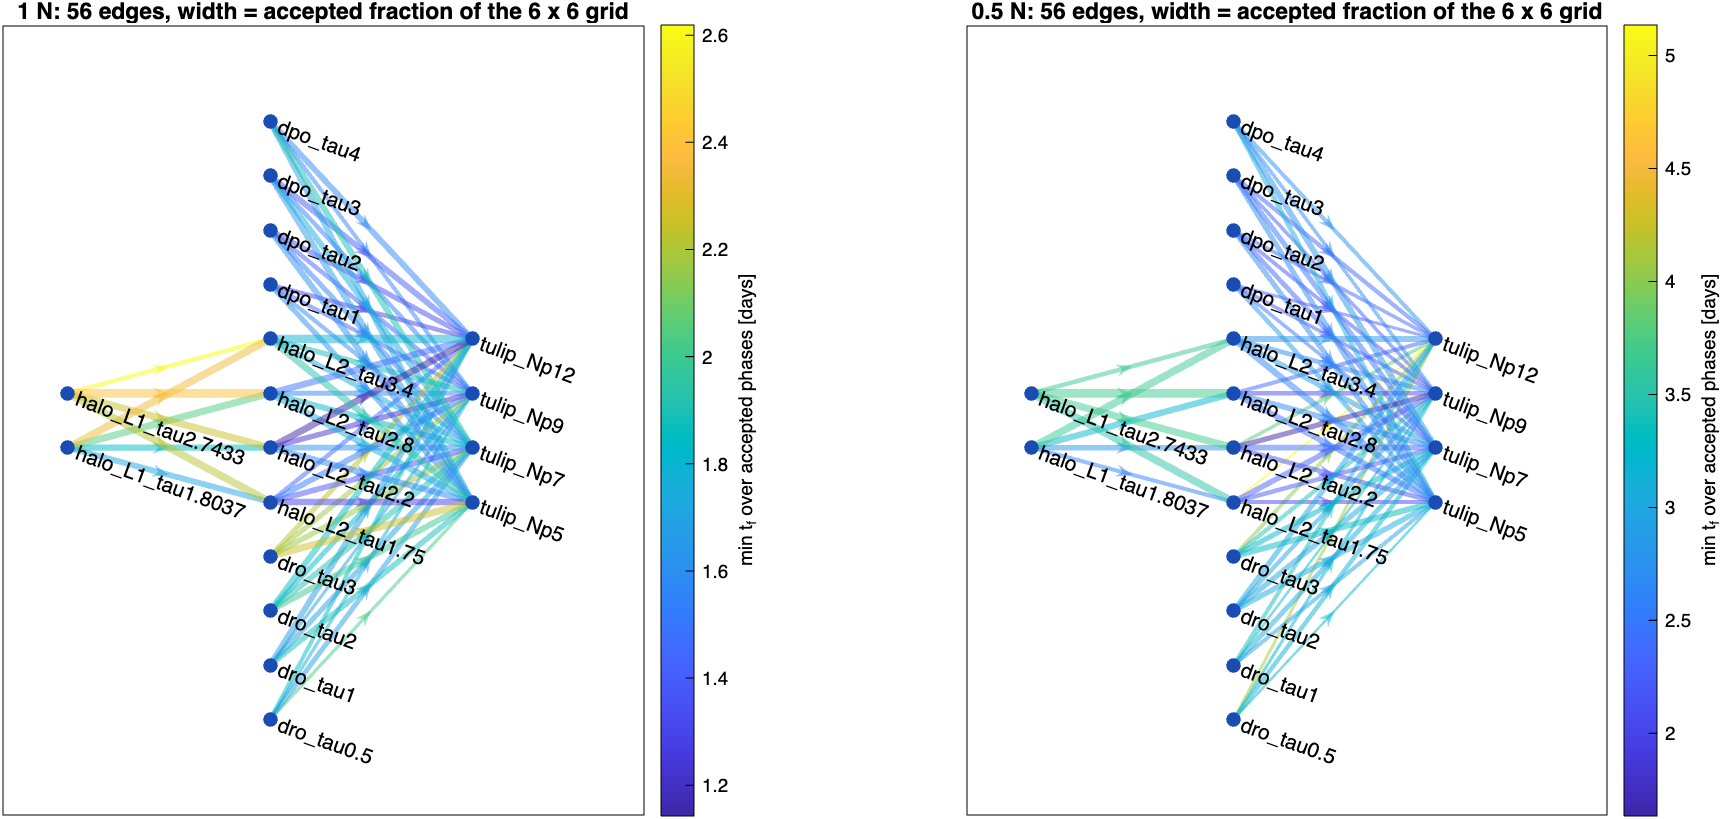
\includegraphics[width=0.78\textwidth]{figures/network_graph.png}
\caption{The network at 1~N (left) and 0.5~N (right): 56 edges, width = accepted fraction of the
$6\times6$ grid, color = minimum $t_f$ over accepted phases.}
\label{fig:graph}
\end{figure}

The strengths at 1~N are the last two columns of Table~\ref{tab:nodes}. They are descriptive only.
Each tulip has 12 in-edges, each L2 halo 2 in and 4 out, and every other orbit 4 out and none in, so
between-family rankings reflect the catalog's topology, not transport. Within a family the numbers
can be compared: among the L2 halos, $\tau = 2.2$ has the largest out-strength (2.949) and
$\tau = 1.75$ the largest in-strength (1.037). Betweenness and weak connectivity are not reported:
only the L2 halos have both in- and out-edges, so either statistic would restate the catalog.

\section{The planes}
Thrust here is a capability axis for one spacecraft, not a consumable budget. Figure~\ref{fig:plane}
reports two planes over (thrust bound, time cap), with 11 rungs and 25 caps from 0.218 to 6.305
days. Raw coverage (left) counts the pairs with an accepted cell at that rung under the cap: what
the catalogs hold at that thrust. The known-feasible envelope (right) counts the pairs with an
accepted cell at that rung or any lower-thrust rung under the cap, since a trajectory accepted at a
lower thrust bound is feasible under a higher one, assuming throttleable thrust at the same specific impulse. The two differ at only two rungs, by one pair
each: at 12~N (37 against 36, cap 0.471~d) and at 3~N (16 against 15, cap 0.725~d).

\begin{figure}[tbp]
\centering
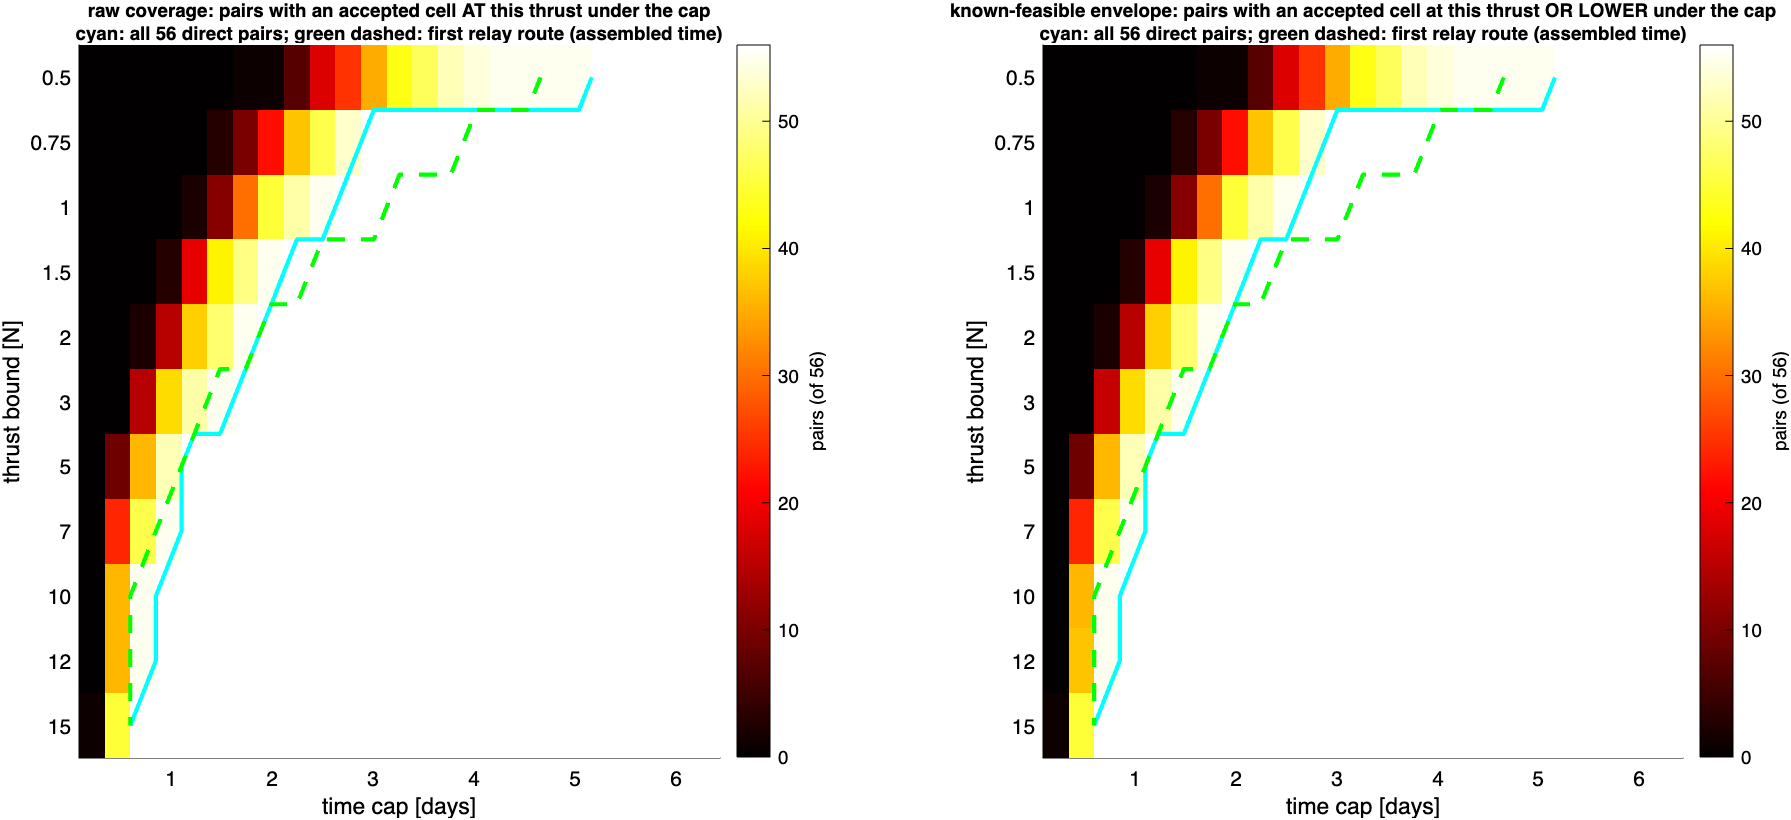
\includegraphics[width=0.7\textwidth]{figures/accessibility_plane.png}
\caption{Raw coverage (left) and the known-feasible envelope (right): pairs with an accepted cell
under the cap. Cyan: all 56 direct pairs covered; green dashed: the first relay route under the
cap, by assembled time.}
\label{fig:plane}
\end{figure}

Two diagnostics are drawn on the planes, and they are diagnostics, not stages. The first is direct
availability, the cyan contour: at 1~N all 56 direct pairs are covered from the first sampled cap
of 2.754 days, and at 0.5~N raw coverage reaches 56 of 56 pairs under the largest cap. The second is
directed reachability with the relay routes of Section~\ref{sec:relay}, the green contour. Of the
306 ordered pairs among 18 orbits, at most $56 + 8 = 64$ are candidates (the direct sheets and the
relay pairs), and at 1~N under the largest cap all 64 are reachable (direct 56 + two-leg 8). On the
sampled caps the first relay route appears at a smaller cap than the last direct pair at 12, 10, 7,
3 and 0.5~N, at the same cap at 15, 5 and 2~N, and at a larger cap at 1.5, 1 and 0.75~N.

Figure~\ref{fig:ladder} shows catalog closure down the ladder: the mean accepted fraction per rung
by departure family. DRO departures fall from 0.858 at 12~N to 0.387 at 0.5~N and DPO departures
from 0.847 to 0.391; L2 halo departures fall from 0.842 to 0.46; L1 halo departures move least,
from 0.767 at 12~N to 0.642 at 0.5~N. The dip at 15~N (smallest for the L1 halos) is the
ladder's starting rung holding fewer cells than 12~N, the coverage fact of Section~\ref{sec:data}.

\begin{figure}[tbp]
\centering
\begin{minipage}[t]{0.49\textwidth}\centering
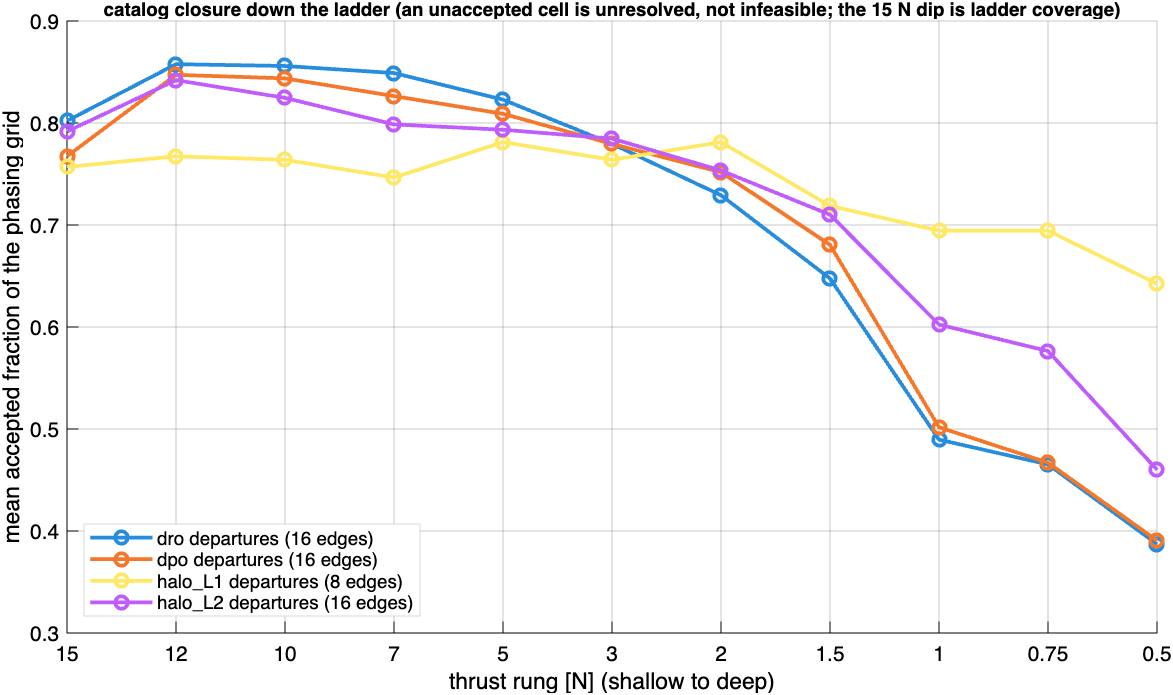
\includegraphics[width=\textwidth]{figures/ladder_closure.png}
\caption{Catalog closure down the ladder: mean accepted fraction of the phasing grid per rung, by
departure family. An unaccepted cell is unresolved, not infeasible.}
\label{fig:ladder}
\end{minipage}\hfill
\begin{minipage}[t]{0.49\textwidth}\centering
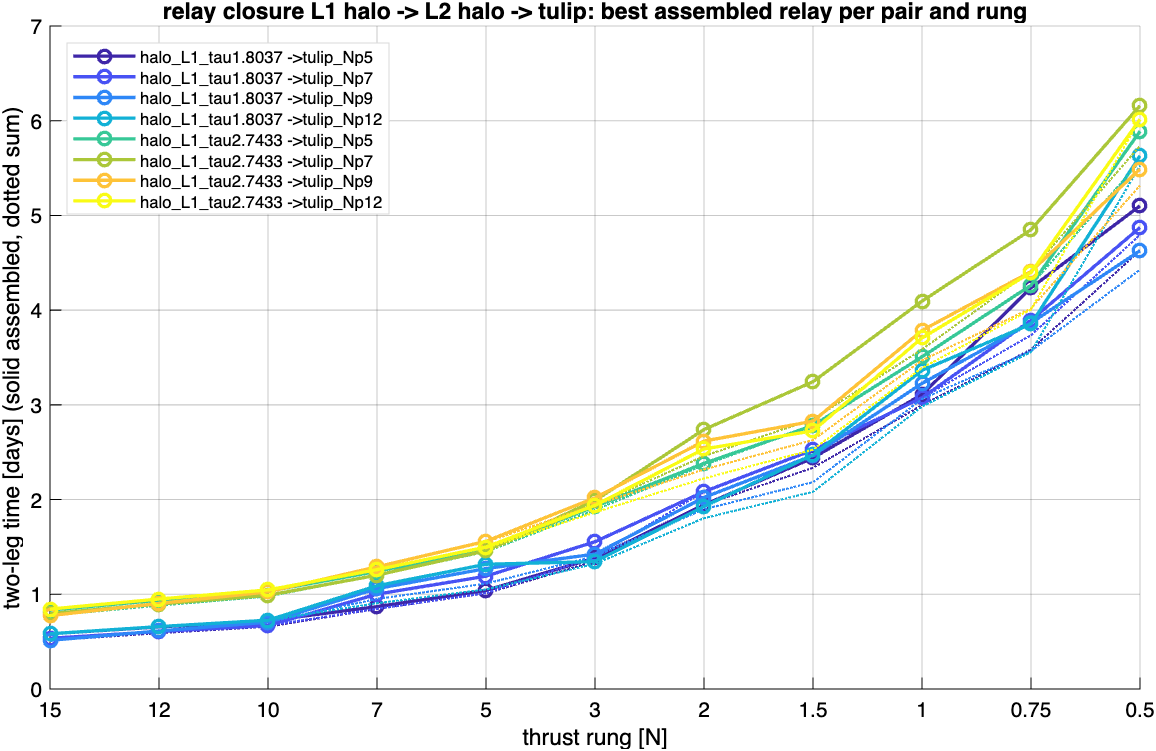
\includegraphics[width=\textwidth]{figures/relay_closure.png}
\caption{Relay closure L1 halo $\to$ L2 halo $\to$ tulip: per pair, the best assembled time
(solid) and the optimistic sum (dotted) against thrust rung.}
\label{fig:relay}
\end{minipage}
\end{figure}

\section{Relay closure}\label{sec:relay}
The only multileg structure in the data is L1 halo $\to$ L2 halo $\to$ tulip: 2 L1 halos, 4 L2
halos and 4 tulips give 32 routes over 8 (L1 halo, tulip) pairs. A route's time is the
phase-compatible assembled time
\[
t_{\mathrm{route}} = \min_{(a,b),\,(c,d)} \Big[\, t_1(a,b) + T_C \,\operatorname{mod}\!\big(s_{D2}(c) - s_{A1}(b),\, 1\big) + t_2(c,d) \Big],
\]
over accepted cells $(a,b)$ of leg 1 and $(c,d)$ of leg 2, where $s_{A1}$ is leg 1's arrival phase
on the relay $C$, $s_{D2}$ leg 2's departure phase on it, and $T_C$ the relay period: the spacecraft
coasts on $C$ from where leg 1 delivers it to where leg 2 starts. The optimistic sum
$t_{\mathrm{sum}} = \min t_1 + \min t_2$ lies beneath it and is kept only as a labelled lower bound.
Both legs use the same phase grid on the relay. All 32 routes find a zero-wait pairing at 1~N (and
at every rung), so the assembled time exceeds the naive sum only through which cells get paired: at
1~N, 7 of the 32 routes have $t_{\mathrm{route}} = t_{\mathrm{sum}}$ (counted over all 32 routes, not read from Table~\ref{tab:relay}). The mass composition of
Section~2 makes every assembled route feasible without a new solve.

\begin{table}[tbp]
\centering\footnotesize
\begin{tabular}{@{}llr>{\raggedleft\arraybackslash}p{4.2cm}r@{}}
\toprule
(L1 halo, tulip) & best relay at 1~N & $t_{\mathrm{route}}$ [d] & smallest optimistic sum over the four relays (pair-level lower bound) [d] & deepest rung \\
\midrule
\texttt{halo\_L1\_tau1.8037}, \texttt{tulip\_Np5}  & \texttt{halo\_L2\_tau1.75} & 3.109 & 2.996 & 0.5~N \\
\texttt{halo\_L1\_tau1.8037}, \texttt{tulip\_Np7}  & \texttt{halo\_L2\_tau1.75} & 3.074 & 3.074 & 0.5~N \\
\texttt{halo\_L1\_tau1.8037}, \texttt{tulip\_Np9}  & \texttt{halo\_L2\_tau1.75} & 3.226 & 3.062 & 0.5~N \\
\texttt{halo\_L1\_tau1.8037}, \texttt{tulip\_Np12} & \texttt{halo\_L2\_tau2.2}  & 3.364 & 2.982 & 0.5~N \\
\texttt{halo\_L1\_tau2.7433}, \texttt{tulip\_Np5}  & \texttt{halo\_L2\_tau1.75} & 3.507 & 3.507 & 0.5~N \\
\texttt{halo\_L1\_tau2.7433}, \texttt{tulip\_Np7}  & \texttt{halo\_L2\_tau1.75} & 4.095 & 3.585 & 0.5~N \\
\texttt{halo\_L1\_tau2.7433}, \texttt{tulip\_Np9}  & \texttt{halo\_L2\_tau2.2}  & 3.786 & 3.470 & 0.5~N \\
\texttt{halo\_L1\_tau2.7433}, \texttt{tulip\_Np12} & \texttt{halo\_L2\_tau2.2}  & 3.706 & 3.390 & 0.5~N \\
\bottomrule
\end{tabular}
\caption{Best relay per (L1 halo, tulip) pair at 1~N by assembled time, and the deepest rung with
any accepted route. The sum column is the smallest optimistic sum over the four relays (a pair-level
lower bound), not the listed relay's own sum.}
\label{tab:relay}
\end{table}

Table~\ref{tab:relay} and Figure~\ref{fig:relay} give the result. All 8 (L1 halo, tulip) pairs
reach 0.5~N by relay. At 1~N, \texttt{halo\_L2\_tau1.75} serves 5 of the 8 pairs as the best
assembled relay and \texttt{halo\_L2\_tau2.2} the other 3; the L2 halos $\tau = 2.8$ and $3.4$ are
never the best. Relay-versus-direct cost is not testable here: no direct L1 halo $\to$ tulip edge
exists, so no pair in the data has both a direct edge and a relay route to compare.

\section{Stability versus cost}
Two responses are computed per sheet over accepted cells: $t_{f1}$, the minimum $t_f$ at 1~N in
days, and the retention to 0.5~N, the fraction of cells accepted at 1~N that are also accepted at
0.5~N. Each is regressed on $\Delta C_J = C_J^{\mathrm{arr}} - C_J^{\mathrm{dep}}$ alone (M0) and on
$\Delta C_J$, $\sigma_{\mathrm{dep}}$ and $\sigma_{\mathrm{arr}}$ (M1), with a partial $F$ test of M1
over M0 and per-coefficient $t$ tests (Figure~\ref{fig:stab}). Braik and Ross's reading predicts a
negative $\sigma_{\mathrm{dep}}$ coefficient for $t_{f1}$ (H1, unstable departures faster) and a
positive one for retention (H2).

For $t_{f1}$, $R^2$ rises from 0.049 (M0) to 0.326 (M1), with partial $F(2,52) = 10.700$,
$p = 0.0001$. The coefficients (nominal OLS, 52 degrees of freedom) are: $\Delta C_J$ $t = -0.17$,
$p = 0.8649$, 95\% CI $[-0.8283, 0.6982]$; $\sigma_{\mathrm{dep}}$ $0.0271$, $t = 0.58$, $p = 0.5656$,
CI $[-0.0670, 0.1213]$; $\sigma_{\mathrm{arr}}$ $0.3785$, $t = 4.33$, $p = 0.0001$, CI
$[0.2032, 0.5539]$. H1: NOT DETECTED (nominal OLS). For retention, $R^2$ rises from 0.111 to 0.164,
partial $F(2,52) = 1.662$, $p = 0.1996$; $\Delta C_J$ $t = -1.48$, $p = 0.1446$, CI
$[-0.7162, 0.1079]$; $\sigma_{\mathrm{dep}}$ $0.0185$, $t = 0.73$, $p = 0.4695$, CI
$[-0.0324, 0.0693]$; $\sigma_{\mathrm{arr}}$ $0.0688$, $t = 1.46$, $p = 0.1510$, CI
$[-0.0259, 0.1634]$. H2: NOT DETECTED (nominal OLS). The group means, descriptive only, are 1.7507
against 1.7467 days for $t_{f1}$ and 0.7767 against 0.8063 for retention (24 stable-departure sheets
against 32 unstable). $\sigma_{\mathrm{arr}}$ varies only on the 8 halo-to-halo sheets, so it is
confounded with that catalog.

Departure instability was not associated with shorter sampled minimum durations or greater catalog
retention at the nominal significance threshold in this exploratory sheet-level model. The time
model's significant joint stability term is associated primarily with arrival instability on the
halo-to-halo sheets. These results neither establish absence of a departure-stability effect nor
test the mechanism in the substantially lower-thrust regime. There are 14 distinct departure orbits
and 8 distinct arrivals; sheets share orbit nodes, and the reported OLS p-values are nominal
model-based summaries. Nonsignificance is not equivalence, and 1~N and 0.5~N sit far above the
70~mN library operating point and the wall between 0.09 and 0.067~N where the catalog's deep DRO
continuation stalls.

\begin{figure}[tbp]
\centering
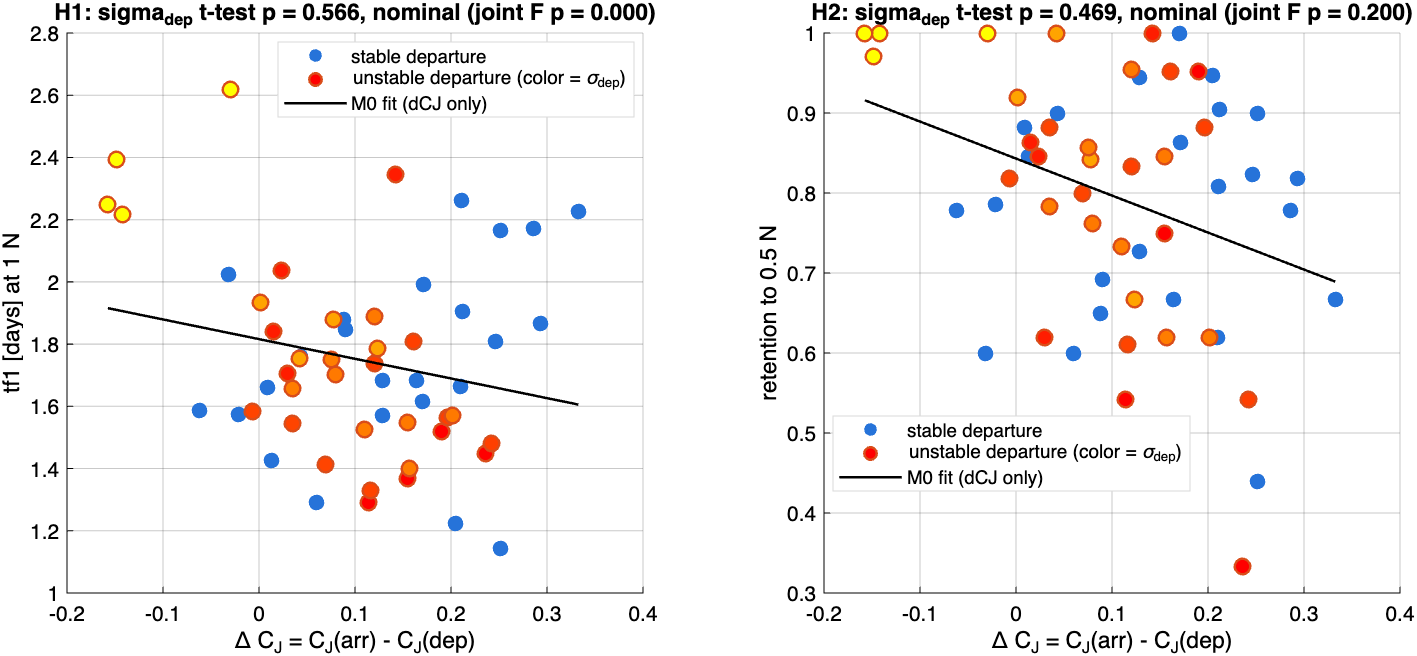
\includegraphics[width=0.5\textwidth]{figures/stability_cost.png}
\caption{Stability versus cost over accepted cells: $t_{f1}$ at 1~N (left) and retention to 0.5~N
(right) against $\Delta C_J$, colored by $\sigma_{\mathrm{dep}}$, with the M0 fit.}
\label{fig:stab}
\end{figure}

\section{The hypothetical reverse graph}
The CR3BP's x-axis symmetry with time reversal,
\[(x,y,z,v_x,v_y,v_z,t) \mapsto (x,-y,z,-v_x,v_y,-v_z,-t),\]
maps a thrusting arc to a thrusting arc,
but of a mass-gain model: the thrust acceleration is reflected by $\mathrm{diag}(1,-1,1)$ and the mass
runs from $m_f$ back to $m_0$. A reversed edge is therefore not a transfer of the physical reverse
problem, not even approximately; it is geometry, carries no certificate, and is off by default. Its
gate G5 checks, for every node, periodic closure $|\phi(x_0,T) - x_0|$ and that the mirror image of
the off-plane state $\phi(x_0, 0.37T)$ lies on the orbit (every stored $x_0$ is on the symmetry
plane, where the mirror check would be vacuous). Both pass at a bar of $10^{-6}$ (closure
$7.6\times10^{-8}$, mirror residual $6.2\times10^{-8}$); the bar is $10^{-6}$ because the
propagator's closure residual on the longest tulip is already $8\times10^{-8}$, while a
perturbed, non-periodic state (2\% in $v_y$) gives $1.4\times10^{-3}$ in the library test. With the reversed edges on (HYPOTHETICAL): 112 edges
($56 + 56$ reversed), one strongly connected component of 18 nodes, and 306 of 306 ordered node
pairs joined by a directed path. These numbers enter no other section or figure.

\section{What the legs campaign would add}
DRO $\to$ DPO and DRO $\to$ L2 halo legs, carried down toward the 70~mN operating point (the
catalog's deep continuation closes 0.09~N and stalls at the wall between 0.09 and 0.067~N), would make DRO $\to$ tulip the
first pair with both a direct edge and a relay route. A relay witness below the direct continuation's
wall would then be a new feasible unrestricted transfer (the lemma), and would say something
about that continuation or the search rather than about a global barrier. The present data supports
candidate prioritization among the L2 halos, from relay usage (Table~\ref{tab:relay}) and the
strengths (Table~\ref{tab:nodes}), not identification of the best DRO relay: the existing
L1 $\to$ L2 legs say nothing about the missing DRO $\to$ L2 leg costs.

The Earth-departure question, how a spacecraft reaches the DRO at all, has no answer in these catalogs;
the nearest existing piece is the GTO $\to$ tulip min-time catalog in \texttt{orbit\_transfer/GTO\_tulip}
(deliverable 7, 16 orientation sheets, with the deep rungs between 3 and 1~N still open; source:
\texttt{GTO\_tulip/catalog/README.md}). This note has not loaded that catalog and has not passed it
through the accepted mask of Section~\ref{sec:data}. If a GTO $\to$ DRO leg were added, GTO
$\to$ tulip would be another pair with both a direct edge and a relay route, beside the DRO
$\to$ tulip pair above. Earth $\to$ DRO $\to$ tulip hopping is therefore a candidate for the legs
campaign; nothing in the present data ranks it against the other candidates.

\begin{thebibliography}{9}
\bibitem{braik2026} S.~Braik and S.~D.~Ross, ``Orbital Networks in the Three-Body Problem,'' arXiv:2605.31543, 2026.
\end{thebibliography}
\end{document}
